\chapter{Evaluation}
In der Evaluation werden drei Aspekte betrachtet: Klassifizierungsgenauigkeit, Robustheit und Resourcennutzung.
Bei der Klassifizierungsgenauigkeit wird einerseits die Standortbestimmung und andererseits die Anomalieerkennung evaluiert.
Dabei wird sowohl auf verschiedene Größen von FFNN und Entscheidungswälder eingegangen,
als auch auf verschieden viele zu unterscheidende Standorte.
\newline
\newline
Bei der Robustheit wird auf den Fehler des besten FFNN und Entscheidungswald bei verschiedene Fehlerszenarien eingegangen.
Diese bestehen aus fehlerhaften Sensordaten durch Rauschen oder ausgefallenen Sensoren und Routen mit permutierten Teilstücken.
\newline
\newline
Bei der Resourcennutzung wird auf die Programmgröße und die Ausführungszeit der besten ML-Modelle eingegangen.
Außerdem wird der Energieverbrauch für verschiedene Szenarien eingeschätzt.
\newline
\newline
Unterschieden werden zwei Varianten der Testmengen.
Diese unterscheiden sich in der Art, wie die Features für den vorherigen Standort bestimmt werden.
In der ersten Variante sind alle vorherigen Standorte korrekt.
In der zweiten Variante ist der erste vorherige Standort als \textit{unbekannt} beschriftet und alle folgenden vorherigen Standorte werden iterativ durch das ML-Modell bestimmt,
d.~h. in dieser Variante wird der propagierte Fehler durch die Rückwärtskante des ML-Modells betrachtet.
Metriken, die auf die zweite Variante der Testmenge angewendet werden sind mit \texttt{cont} markiert.

\section{Metriken}
In dieser Arbeit werden verschiedene Metriken zur Ermittlung der Klassifizierungsgenauigkeit ermittelt.
Zunächst die übliche Klassifizierungsgenauigkeit (\ref{formular:simple_accuracy}), in der die Anzahl der korrekt klassifizierten Standorte mit der Gesamtanzahl verglichen werden.
\begin{align}
    \label{formular:simple_accuracy}
    P(A) := \frac{\text{Anzahl korrekter Klassifizierungen}}{\text{Gesamtanzahl}}
\end{align}
Die zweite Metrik (\ref{formular:accuracy_metrik2}) betrachtet die Klassifizierungsgenauigkeit unter Tolerierung, dass ein Standort
fünf bzw. zehn Klassifizierungen kontinuierlich zu früh oder zu spät verlassen wurde,
d.~h. Fehlklassifizierungen werden vernachlässigt, wenn kontinuierlich der letzte korrekte Standort bzw. der nächste korrekte
Standort klassifiziert wird mit einer Gesamttoleranz von fünf bzw. zehn Klassifizierungen.
\begin{flalign}
    \label{formular:accuracy_metrik2}
    &\epsilon \in \{5, 10\} \nonumber\\
    &L := \text{Menge von dem ML-Modell klassifizierten Standorte.} \nonumber\\
    &K := \text{Menge von den wirklichen Standorten.} \nonumber\\
    &\Phi(i) := \text{Index von dem nächsten Standort.} \nonumber\\
    &\Psi(i) := \text{Index von dem vorherigen Standort.} \nonumber\\
    &\Omega(i) := \Phi(i)-i\leq\epsilon\wedge\hspace{-0.3cm} \bigwedge\limits_{i\leq q \leq \min(\#K, \Phi(i))}\hspace{-0.3cm} L_q=K_{\Phi(i)} \nonumber\\
    &\Theta(i) := i-\Psi(i)\leq\epsilon\wedge\hspace{-0.3cm} \bigwedge\limits_{\max(0, \Psi(i))\leq q \leq i}\hspace{-0.3cm} L_q=K_{\Psi(i)} \nonumber\\
    &P(B) := \frac{\#\{L_i | L_i=K_i \vee \Omega(i) \vee \Theta(i)\text{ für } i\in\{0, 1, ..., \#L - 1\}\}}{\#K}
\end{flalign}
Zuletzt zwei Metriken bei denen die Klassifizierungsgenauigkeit bestimmt wird, unter der Bedingung, dass der vorherige
Standort korrekt (\ref{formular:accuracy_previous_was_correct}) bzw. falsch (\ref{formular:accuracy_previous_was_wrong}) war.
\begin{align}
    \label{formular:accuracy_previous_was_correct}
    P(C) := \frac{\text{Anzahl korrekter Klassifizierungen, wenn vorheriger Standort korrekt war}}{\text{Alle Klassifizierungen, wenn vorheriger Standort korrekt war}}
\end{align}
\begin{align}
    \label{formular:accuracy_previous_was_wrong}
    P(D) := \frac{\text{Anzahl korrekter Klassifizierungen, wenn vorheriger Standort falsch war}}{\text{Alle Klassifizierungen, wenn vorheriger Standort falsch war}}
\end{align}
\section{Klassifizierungsgenauigkeit der Standorte}
Die Klassifizierungsgenauigkeit der ML-Modelle zur Standorterkennung wurde mit verschiedenen Konfigurationen über komplexer werdende Datenmengen evaluiert.
In Kapitel \ref{sec:model_dt} und Kapitel \ref{sec:model_ffnn} werden die einzelnen Konfigurationen der ML-Modelle beschrieben.
Die Komplexität wird über die Anzahl der Standorte definiert.
Um die Anzahl der Standorte zu erhöhen, wurden die Datenmengen um weitere Routen erweitert.
Dies impliziert aber, dass die Testmengen nicht vergleichbar sind unter den Standortanzahlen, da mit jeder Route auch die Testmenge erweitert wird.
Die berechneten Klassifizierungswahrscheinlichkeiten sind jeweils der Durchschnitt der Klassifizierungswahrscheinlichkeiten aller Routen in der Testmenge.
\newline
\newline
Außerdem unterscheiden sich die Enkodierungsansätze je nach Standortanzahl.
Für die Standortanzahlen 9, 17, 25 und 52 wurde der Enkodierungsansatz verwendet, bei denen nur die Knoten und ein zusätzlicher unbekannter Standort betrachtet wird.
Für die Standortanzahlen 16, 32, 48 und 102 wurde der Enkodierungsansatz verwendet, bei denen Knoten und Kanten betrachtet werden.
Ein besserer Ansatz, um Daten mit beliebiger Komplexität zu generieren wird in Kapitel \ref{chapter:discussion} diskutiert.
\newline
\newline
Zunächst wird die Klassifizierungsgenauigkeit $P(A)$ im Vergleich zu Mians Ergebnissen betrachtet.
Mian konnte mit einem WFFNN bei einer Route mit drei Pfaden und 14 Standorten eine Klassifizierungsgenauigkeit von 94,1\% erreichen \cite{naveedThesis}.
Abbildung \ref{fig:best_dt_acc_vs_knn_acc_vs_cont} vergleicht die Klassifizierungsgenauigkeiten der
Entscheidungsbaum basierten Klassifizierer und FFNN über verschiedene Standortkomplexitäten.
Dabei wurde stets die höchste Klassifizierungsgenauigkeiten aller evaluierten Konfigurationen ausgewählt.
Gezeigt werden sowohl die Klassifizierungsgenauigkeiten auf die Testmengen die korrekt beschriftet sind und die, die von den ML-Modellen beschriftet sind.
\begin{figure}[h!]
    \centering
    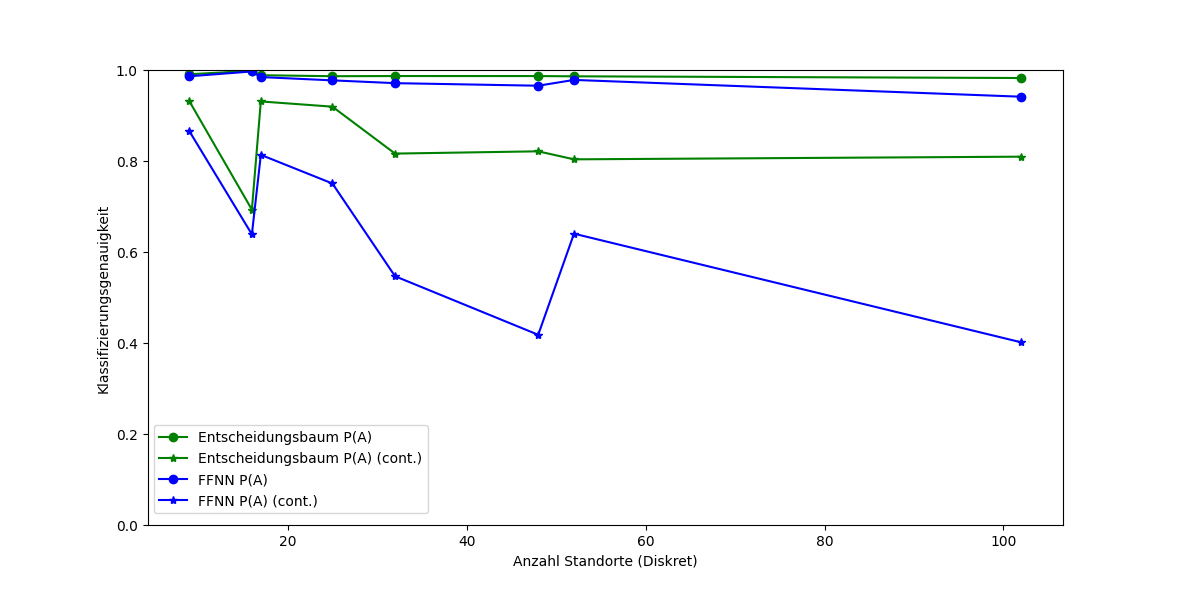
\includegraphics[width=\linewidth]{images/best_dt_vs_knn_acc_vs_acc_cont.png}
    \caption{Die besten Klassifizierungsgenauigkeiten aller evaluierten Konfigurationen der ML-Modelle über alle Standortkomplexitäten.}
    \label{fig:best_dt_acc_vs_knn_acc_vs_cont}
\end{figure}
\newline
\newline
Mian hat in seiner Evaluation die Klassifizierungsgenauigkeit $P(A)$ betrachtet.
Die in dieser Arbeit evaluierten Standortkomplexität, die Mians Evaluation am nächsten kommt ist 16.
Im Vergleich ist der beste Entscheidungsbaum basierte Klassifizierer mit einer Klassifizierungsgenauigkeit von 99,9\%, 5,8 Prozentpunkte besser
und das beste FFNN mit einer Klassifizierungsgenauigkeit von 99,79\%, 5,69 Prozentpunkte besser (Tabelle \ref{tab:predictions_by_acc}).
\newline
\newline
Dies betrachtet aber nicht den propagierten Fehler, der durch die Rekursion der ML-Modelle entsteht.
In Abbildung \ref{fig:best_dt_acc_vs_knn_acc_vs_cont} ist zu sehen, dass die Klassifizierungsgenauigkeit signifikant geringer ist bei allen Standortkomplexitäten.
Besonders mit der Standortkomplexität 16 ist die Klassifizierungsgenauigkeit signifikant geringer, wobei dies eine Artefakt der Enkodierungsmethode sein kann,
da bei der Standortkomplexität 17 immernoch Entscheidungsbaum basierte Klassifizierer mit einer Klassifizierungsgenauigkeit von 95,86\% gefunden wurden (Tabelle \ref{tab:predictions_by_acc_cont}).
Die FFNNS hingegen erreichen lediglich maximal 88,1\% bei dieser Standortkomplexität.
\newline
\newline
Aus Tabelle \ref{tab:predictions_by_acc_10_cont} können die Klassifizierungsgenauigkeiten $P(B=10)$ entnommen werden.
Der Entscheidungsbaum basierte Klassifizierer skaliert dabei sehr gut mit der steigenden Standortkomplexität.
Aber einer Standortkomplexität von 32 wird konnte aber nurnoch eine Klassifizierungsgenauigkeit von 91,35\% erreicht werden, die bis auf 87,87\% bei 102 Standorten fällt.
Als beste maximale Baumhöhe hat sich 16 herausgestellt, wobei 32 und 64 marginal schlechtere Ergebnisse produzierten.
Eine maximale Baumhöhe von 8 war nicht ausreichend und hat sich hat deutlich schlechtere Ergebnisse erzielt.
Bei gleicher Waldgröße haben die maximalen Baumhöhen und 32 und 64 equivalente Ergebnisse produziert.
Die verschiedenen Waldgrößen unterscheiden sich nicht stark.
Eine Waldgröße von 8 hat nur marginal schlechtere Ergenisse bei 102 Standorten erzielt, als die Waldgrößen 16, 32 und 64.
Aus diesem Grund ist eine Waldgröße von 8 ausreichend, oder könnte womöglich immernoch reduziert werden.
\newline
\newline
Die evaluierten FFNNs skalieren deutlich schlechter als die Entscheidungsbaum basierten Klassifizierer mit steigender Standortkomplexität.
Besonders die FFNNs der Standortkomplexitäten, die das Enkodierungsverfahren der Kanten und Knoten nutzte,
konnten signifikant schlechtere Klassifizierungsergebnisse erzielen als die FFNNs die das andere Enkodierungsverfahren nutzten.
Aus den Daten ist nicht zu schließen, wie sich die Anzahl der Schichten und Neuronen pro Schicht auf die Klassifizierungsgenauigkeit auswirkt.
Für geringe Standortkomplexitäten haben vermehrt kleine FFNNs besser abgeschnitten und für große Standortkomplexitäten vermehrt große FFNNs.
\begin{table}[h!]
    \hspace{-1.5cm}
    \begin{tabular}{ | c | c | c | c | c | c | c | c | c | c | }
        \hline
        \multicolumn{2}{ | l |}{$P(B=10)_{\text{cont}}$ über Standorte} & 9 & 16 & 17 & 25 & 32 & 48 & 52 & 102 \\\hline
        \multicolumn{10}{| l |}{\textbf{Entscheidungswälder}}\\\hline
        Waldgröße & Max. Baumgröße & \multicolumn{8}{ c |}{}\\\hline
        16 & 8 & 99.88 & 81.69\% & 99.50\% & 94.21\% & 82.88\% & 88.40\% & 85.72\% & 79.01\% \\\hline
        16 & 16 & 99.78 & 77.30\% & 99.73\% & 93.40\% & 91.35\% & 92.86\% & 89.86\% & 89.10\% \\\hline
        16 & 32 & 99.78 & 77.00\% & 99.83\% & 98.31\% & 86.55\% & 92.60\% & 90.66\% & 85.69\% \\\hline
        16 & 64 & 99.78 & 77.00\% & 99.83\% & 98.31\% & 86.55\% & 92.60\% & 90.66\% & 85.69\% \\\hline
        8 & 32 & 98.92 & 92.79\% & 99.66\% & 98.10\% & 90.27\% & 91.45\% & 89.46\% & 85.11\% \\\hline
        16 & 32 & 99.78 & 77.00\% & 99.83\% & 98.31\% & 86.55\% & 92.60\% & 90.66\% & 85.69\% \\\hline
        32 & 32 & 99.79 & 78.06\% & 99.63\% & 97.52\% & 88.83\% & 93.33\% & 89.20\% & 86.92\% \\\hline
        64 & 32 & 99.69 & 84.66\% & 99.82\% & 97.62\% & 89.65\% & 93.31\% & 86.15\% & 87.87\% \\\hline
        32 & 64 & 99.79 & 78.06\% & 99.63\% & 97.52\% & 88.83\% & 93.33\% & 89.20\% & 86.92\% \\\hline
        \multicolumn{10}{| l |}{\textbf{Feed Forward neuronale Netzwerke}}\\\hline
        \#Schichten & \#Neuronen & \multicolumn{8}{ c |}{}\\\hline
        1 & 16 & 99.65 & 76.69\% & 93.25\% & 83.76\% & 45.93\% & 65.16\% & 76.85\% & 42.39\% \\\hline
        1 & 32 & 99.77 & 77.04\% & 93.47\% & 84.28\% & 63.63\% & 64.21\% & 76.40\% & 44.73\% \\\hline
        1 & 64 & 99.69 & 68.52\% & 95.35\% & 88.93\% & 50.44\% & 83.60\% & 80.52\% & 33.87\% \\\hline
        1 & 128 & 99.10 & 75.39\% & 92.96\% & 91.02\% & 52.27\% & 55.62\% & 82.18\% & 42.56\% \\\hline
        2 & 32 & 98.59 & 63.99\% & 96.98\% & 87.72\% & 68.52\% & 73.21\% & 79.07\% & 35.48\% \\\hline
        4 & 32 & 99.61 & 71.53\% & 93.63\% & 93.19\% & 49.47\% & 52.64\% & 82.16\% & 38.66\% \\\hline
        8 & 32 & 92.74 & 62.31\% & 86.52\% & 86.57\% & 36.36\% & 71.92\% & 75.98\% & 51.15\% \\\hline
        4 & 64 & 99.06 & 67.74\% & 93.76\% & 94.15\% & 54.47\% & 47.75\% & 82.08\% & 47.55\% \\\hline
    \end{tabular}
    \caption{Metrik $P(B=10)_{\text{cont}}$ über Standorte und verschiedenen Konfigurationen der ML-Modelle.}
    \label{tab:predictions_by_acc_10_cont}
\end{table}
\section{Klassifizierungsgenauigkeit der Anomalien}
\label{sec:eval_anomalieerkennung}
Bei der Anomalieerkennung werden Entscheidungswälder und FFNNs mit den besten ML-Modellen zur Standorterkennung trainiert und mit den drei Baseline-Modellen verglichen.
Tabelle \ref{tab:anomaly_detection_prediction_accuracy} zeigt die Klassifizierungsgenauigkeiten über die verschiedenen Standortkomplexitäten,
wobei die Klassifizierungsgenauigkeit $P(A)$ nochmal genauer aufgeschlüsselt ist in den Anteil der korrekten Klassifizierungen, wenn eine bzw. keine Anomalie vorlag.
Die trainierten FFNNs geben stets aus, dass keine Anomalie vorliegt.
Es ist unklar, warum die FFNNs sich so verhalten.
\begin{table}[h!]
    \hspace{-1cm}
    \begin{tabular}{ | l | c | c | c | c | c | c | c | c | }
        \hline
        Standorte & 9 & 16 & 17 & 25 & 32 & 48 & 52 & 102 \\\hline
        \multicolumn{9}{ | l |}{$P(A)$}\\\hline
        Entscheidungswald & 82,59\% & 81,19\% & 87,14\% & 84,91\% & 79,06\% & 83,47\% & 81,93\% & 76,00\% \\\hline
        FFNN & 77,88\% & 77,88\% & 77,88\% & 77,88\% & 77,88\% & 77,88\% & 77,88\% & 77,88\% \\\hline
        Topologie (DT) & 84,77\% & 30,57\% & 83,51\% & 79,76\% & 28,63\% & 24,97\% & 80,55\% & 29,47\% \\\hline
        Topologie (KNN) & 86,10\% & 52,17\% & 77,72\% & 79,30\% & 45,06\% & 41,92\% & 74,77\% & 43,55\% \\\hline
        \multicolumn{9}{ | l |}{Anteil korrekt klassifiziert, indem Anomalie vorlag}\\\hline
        Entscheidungswald & 34,86\% & 35,52\% & 52,58\% & 50,92\% & 32,21\% & 50,64\% & 23,21\% & 1,92\% \\\hline
        FFNN & 0,00\% & 0,00\% & 0,00\% & 0,00\% & 0,00\% & 0,00\% & 0,00\% & 0,00\% \\\hline
        \multicolumn{9}{ | l |}{Anteil korrekt klassifiziert, indem keine Anomalie vorlag}\\\hline
        Entscheidungswald & 96,14\% & 94,41\% & 97,05\% & 95,83\% & 92,48\% & 93,13\% & 98,96\% & 97,18\% \\\hline
        FFNN & 100,00\% & 100,00\% & 100,00\% & 100,00\% & 100,00\% & 100,00\% & 100,00\% & 100,00\% \\\hline
    \end{tabular}
    \caption{$P(A)$ über Standorte und Modelle zur Anomalieerkennung.}
    \label{tab:anomaly_detection_prediction_accuracy}
\end{table}
\newpage
Die Entscheidungswälder hingegen eignen sich besser für den Anomalieerkennungszweck.
Es werden zwischen 1,92\% und 52,58\% der Anomalien erkannt und zwischen 1,04\% und 7,52\% falsch als Anomalien erkannt.
Die Klassifizierungsgenauigkeit des Entscheidungswaldes zur Anomalieerkennung ist abhängig von der Klassifizierungsgenauigkeit zur Standorterkennung
und von der Standortkomplexität.
Je besser das Standorterkennungsmodell und je höher die Standortkomplexität, desto höher ist die Anomalieerkennungsrate.
Aus diesem Grund ist die Klassifizierungsgenauigkeit bei den Standortkomplexitäten, die mit der Kodierungsmethode mit Kanten und Knoten zusammenhängen,
geringer, als bei der Kodierungsmethode, bei der nur die Knoten kodiert werden.
\newline
\newline
Abbildung \ref{fig:true_vs_predicted_anomaly} zeigt einen Auscchnitt der Anomalietestmenge, worauf der Entscheidungswald der Standortkomplexität 17 angewendet wurde.
Die Anomalie wird nicht kontinuierlich erkannt und es werden auch fälschlicherweise Standorte als Anomalien klassifiziert.
Allerdings treten falsch-positive Ergebnisse nur vereinzelt auf, wohingegen bei einer Anomalie, sehr häufig eine Anomalie erkannt wird.
Die falsch-positiven Ergebnisse können somit durch Ausnutzen dieser Fluktuationen vermieden werden,
indem beispielweise ein Schwellenwert an Ausschlägen in einer bestimmten Zeit eingeführt wird.
\begin{figure}[h!]
    \centering
    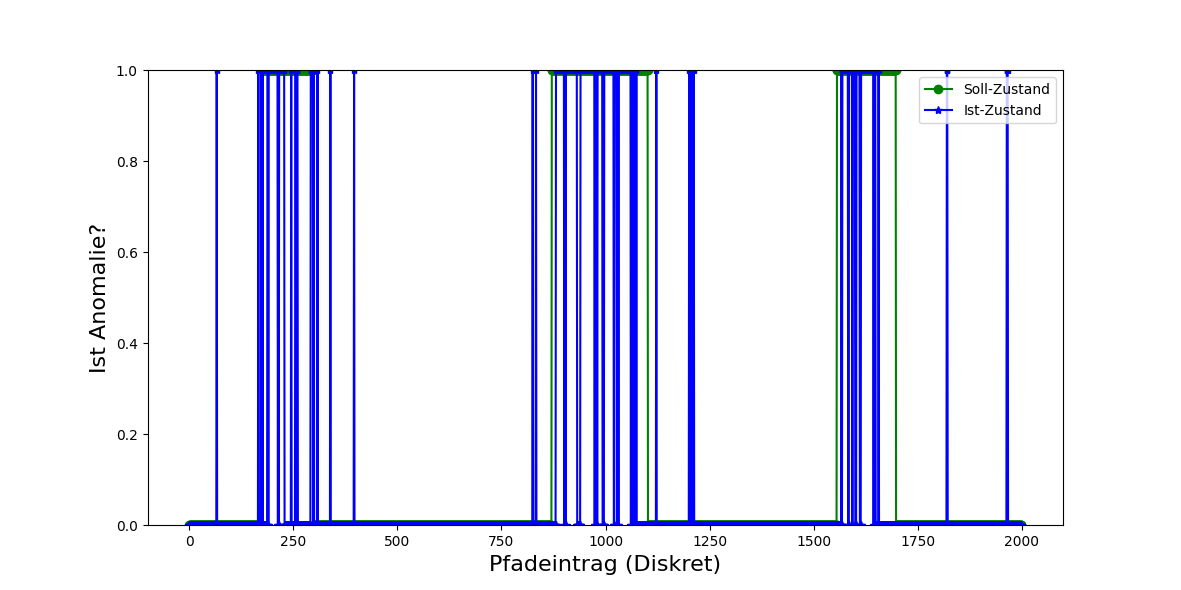
\includegraphics[width=\linewidth]{images/anomaly_true_vs_predicted.png}
    \caption{Ausschnitt der Klassifizierungsergebnisse auf der Anomalietestmenge mit dem Entscheidungswald der Standortkomplexität 17. }
    \label{fig:true_vs_predicted_anomaly}
\end{figure}
\section{Signifikanz der Features}
Die Signifikanz der Features wird über die Permutationswichtigkeit bestimmt.
Die Permutationswichtigkeit ist der Fehler, der durch das permutieren eines Features in der Testmenge entsteht, im Vergleich zu der ursprünglichen Testmenge.
Je größer der Fehler, desto wichtiger das Feature.
\newline
\newline
Abbildungen \ref{fig:feature_significance_dt} und \ref{fig:feature_significance_knn} zeigen die Permutationswichtigkeit eines Entscheidungswaldes und FFNN.
Die Permutationswichtigkeit von einzelnen Entscheidungswäldern bzw. FFNNs unterscheidet sich nicht stark.
Beide ML-Modelle weisen den vorherigen Standorten eine hohe Signifikanz zu.
Die Klassifizierunggenauigkeiten in Tabelle \ref{tab:predictions_by_acc_pic_cont} bestätigen diese Abhängigkeit.
Demnach ist die Wahrscheinlichkeit sehr gering, dass der Standort korrekt klassifiziert wird, wenn der vorherige Standort inkorrekt war.
\begin{figure}[h!]
    \centering
    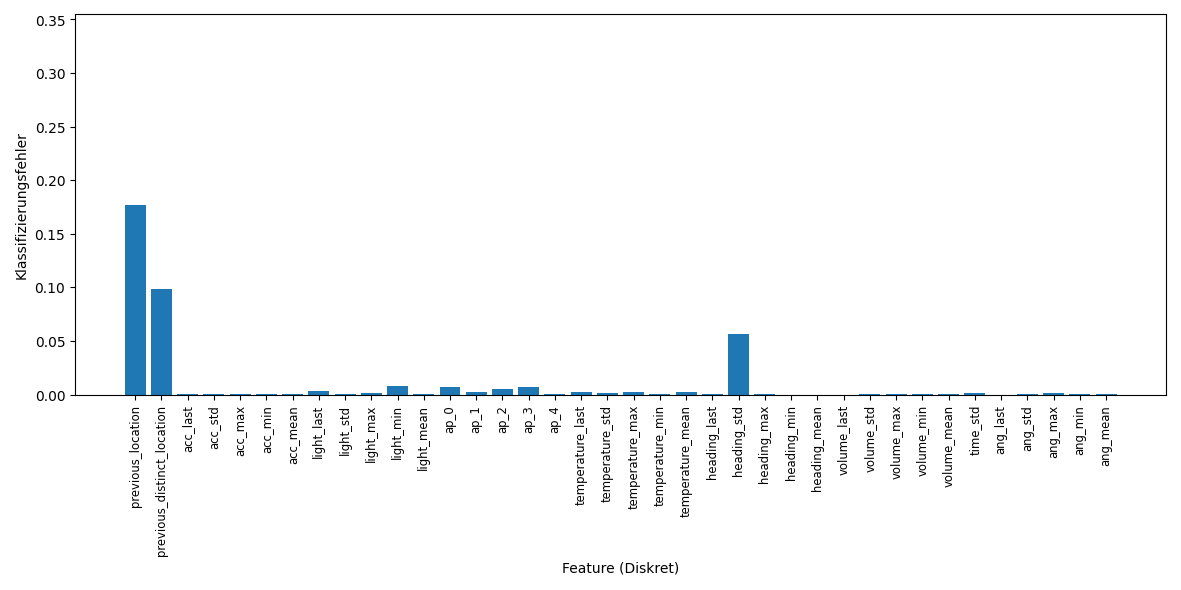
\includegraphics[width=\linewidth]{images/evaluation_feature_importance_dt_pi.png}
    \caption{Permutationswichtigkeit der Features eines Entscheidungswaldes.}
    \label{fig:feature_significance_dt}
\end{figure}
\begin{figure}[h!]
    \centering
    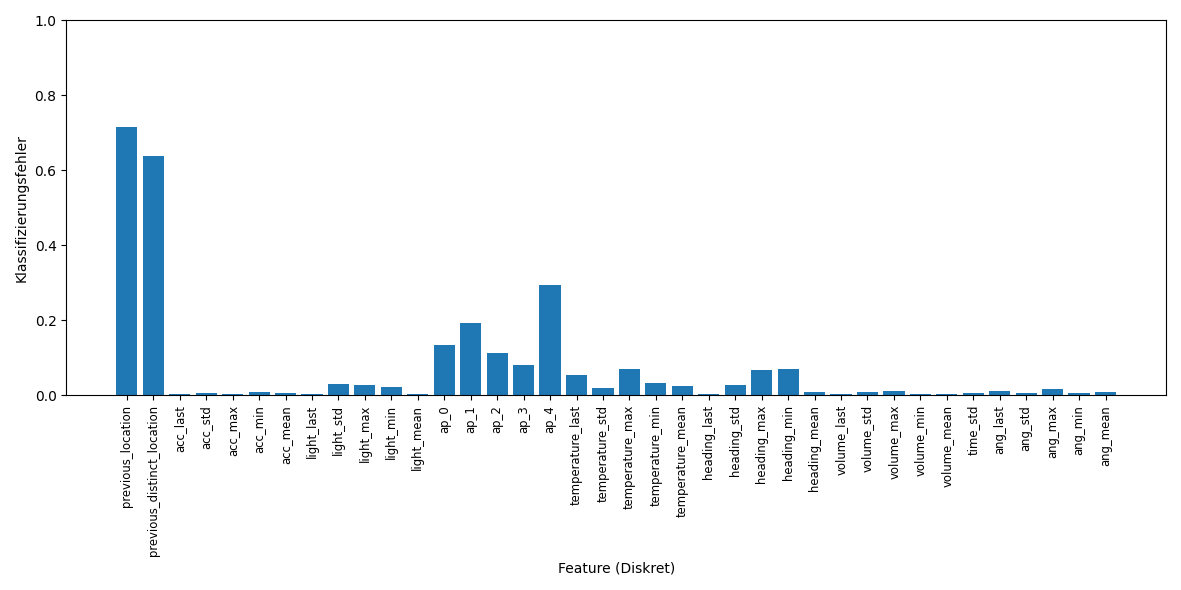
\includegraphics[width=\linewidth]{images/evaluation_feature_importance_knn_pi.png}
    \caption{Permutationswichtigkeit der Features eines FFNN.}
    \label{fig:feature_significance_knn}
\end{figure}
\newline
\newline
Für die Entscheidungswälder sind alle Features, bis auf die vorherige Position und die Standardabweichung in der Ausrichtung zum Magnetfeld unwichtig.
Die FFNNs hingegen bedienen sich außerdem Features von dem Temperatursensor, dem Lichtsensor und vor allem der Detektierung von WLAN-Zugangspunkten.
Allerdings sind FFNNs deutlich abhängiger von dem vorherigen Standort als Entscheidungswälder.
\newline
\newline
Durch diese Abhängigkeit ist keine hohe Robustheit zu erwarten der ML-Modelle zu erwarten.
Diese Abhängigkeit ließe sich Eliminieren, indem ohne die Rückwärtskante trainiert wird.
Dies simplifiziert den Trainingsprozess, wodurch die ML-Modelle schneller zu trainieren sind.
Tabelle \ref{tab:predictions_wo_feedback_edge_by_acc} zeigt, dass diese ML-Modelle vergleichbare Klassifizierungsgenauigkeiten erzielen.
Insbesondere FFNNs erzielen deutlich bessere Klassfizierungsgenauigkeiten, erzielen aber dennoch schlechtere Ergebnisse als die Entscheidungswälder.
Hier ist die Metrik $P(A)$ mit der Metrik $P(A)_{\text{cont}}$ vergleichbar, da der propagierte Fehler durch die Eliminierung der Rückwärtskante nicht mehr existiert.
\newline
\newline
Abbildungen \ref{fig:feature_significance_dt_wo_fe} und \ref{fig:feature_significance_knn_wo_fe} zeigen die Permutationswichtigkeit der ML-Modelle ohne Rückwärtskante.
Beide ML-Modelle gewichten Features aus anderen Sensorwerten deutlich mehr, im Vergleich zu den ML-Modellen mit Rückwärtskante.
Die Entscheidungswälder gewichten dennoch nur die Standardabweichung der Ausrichtung zum Magnetfeld, due Detektierung der WLAN-Zugangspunkte und das Minimum des Lichtsensors stark.
Die anderen Features sind im Vergleich deutlich unwichtiger.
Das FFNN hingegen nutzt alle Features, wobei Features aus dem Accelerometer und Gyroskop unwichtiger sind.
\begin{figure}[h!]
    \centering
    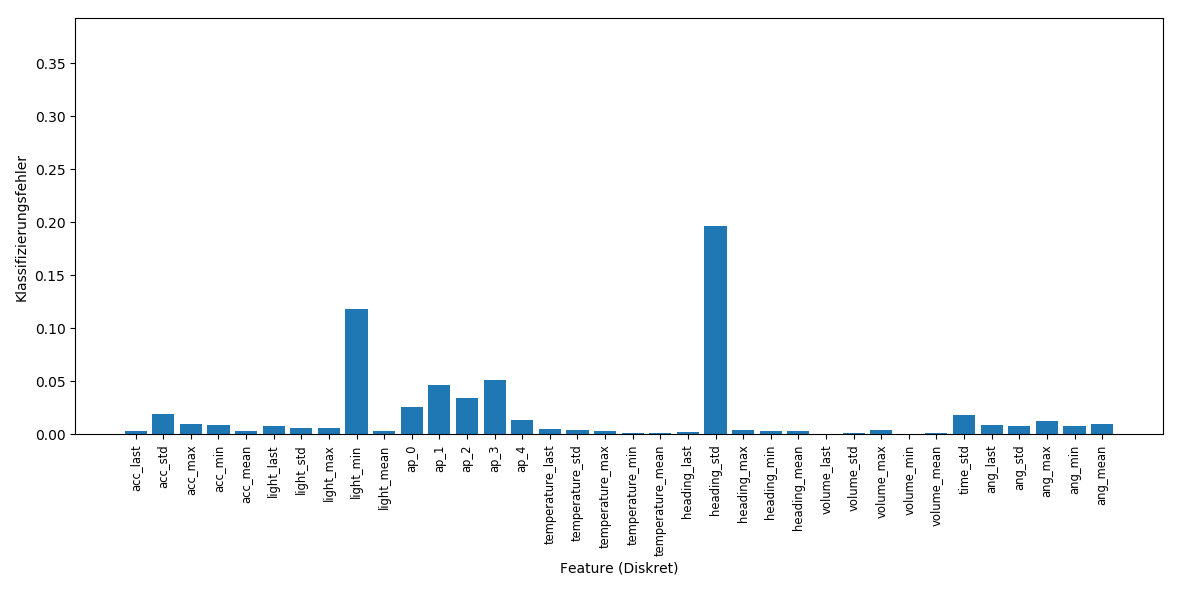
\includegraphics[width=\linewidth]{images/fi_wo_fe_dt.png}
    \caption{Permutationswichtigkeit der Features eines Entscheidungswaldes ohne Rückwärtskante.}
    \label{fig:feature_significance_dt_wo_fe}
\end{figure}
\begin{figure}[h!]
    \centering
    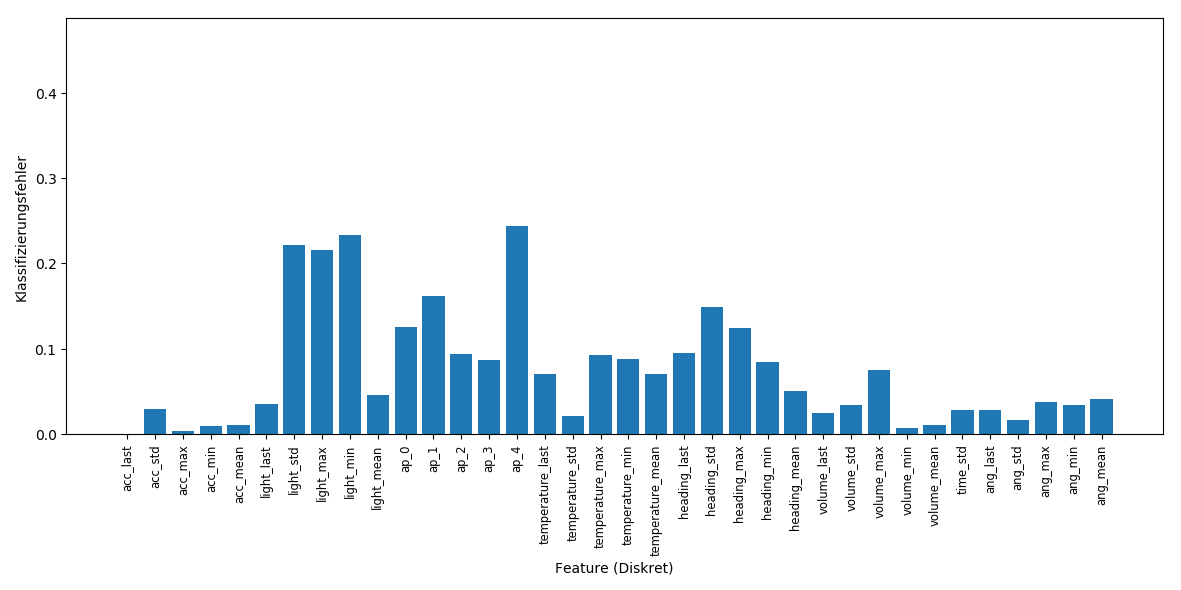
\includegraphics[width=\linewidth]{images/fi_wo_fe_knn.png}
    \caption{Permutationswichtigkeit der Features eines FFNN ohne Rückwärtskante.}
    \label{fig:feature_significance_knn_wo_fe}
\end{figure}
\section{Benötigte Trainingsdaten}
Mit wachsender Standortkomplexität werden mehr Trainingsdaten benötigt.
Abbildung \ref{fig:required_training_data} zeigt die benötigten Trainingszyklen für Entscheidungswälder und FFNNs mit Rückwärtskante bis auf der Testmenge
eine Klassifizierungsgenauigkeit $P(A)$ von 97\% erreicht wurde.
Es wurde 97\% als Grenze gewählt, da 97,26\% die höchste Klassifizierungsgenauigkeit des FFNNs bei einer Standortkomplexität von 102 ist.
Die Trainingszyklen korrelieren mit der Anzahl der Trainingsdaten, da mit jedem Zyklus die Trainingsdaten ergänzt werden.
\begin{figure}[h!]
    \centering
    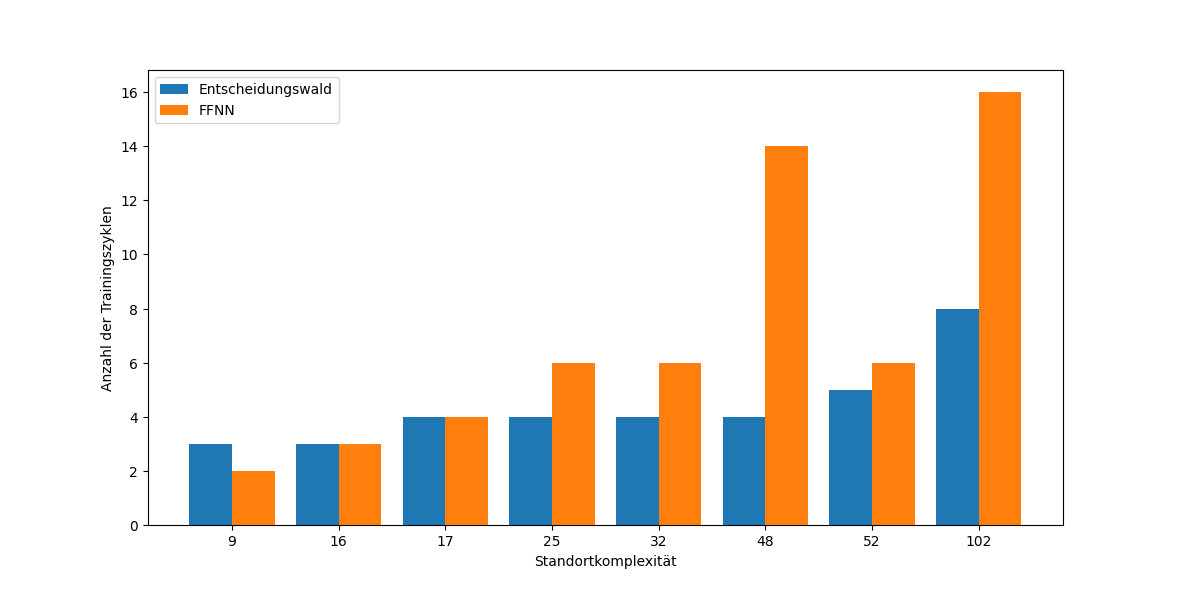
\includegraphics[width=\linewidth]{images/required_training_data.png}
    \caption{Anzahl der benötigten Trainingszyklen bis $P(A)=97\%$ auf der Testmenge erreicht wurde. }
    \label{fig:required_training_data}
\end{figure}
\newline
\newline
Die Entscheidungswälder benötigen weniger Trainingszyklen als FFNNs, um den Schwellenwert zu erreichen.
Je größer die Standortkomplexität, desto größer wird die Differenz der benötigten Trainingsdaten.
Die ML-Modelle ohne Rückwärtskante wurden nicht in Zyklen trainiert, weswegen keine Aussage über die benötigten Trainingsdaten getroffen wird.
\section{Fehlertoleranz}
Bei der Fehlertoleranz wird die Fähigkeit der ML-Modelle untersucht, trotz fehlerhafter Sensordaten Standorte zu erkennen.
Dafür wurden für jeden Sensor modifizierte Testmengen erstellt.
Die erste Testmenge fügt ein Rauschen von 5\% hinzu und die zweite Testmenge simuliert den Ausfall des Sensors, indem alle Sensorwerte genullt werden.
Zudem wurde untersucht, was passiert wenn die Sensorenbox nicht dem trainierten Pfad folgt, indem die Testmenge permutiert wurde.
Damit Entscheidungswald und FFNN fair verglichen werden können, werden die besten ML-Modelle der Standortkomplexität 9 verwendet.
\newline
\newline
Tabelle \ref{tab:robustness} zeigt die Differenz der Klassifizierungsgenauigkeiten $P(A)_{\text{cont}}$ und $P(A)$ von den modifizierten Testmengen zur originalen Testmenge.
Die Testmengen mit einem Rauschen von 5\% wurde ausgelassen, da es keine Auswirkung auf die Klassifizierungsgenauigkeit hatte.
Vermutlich ist 5\% Rauschen zu wenig, um einen Einfluss auszuüben.
\begin{table}[h!]
    \hspace{-1.25cm}
    \begin{tabular}{ | l | c | c | c | c | }
        \hline
        Testmenge & Entscheidungswald & FFNN & Entscheidungswald & FNNN \\\hline
        & \multicolumn{2}{ c }{mit Rückwärtskante} & \multicolumn{2}{| c |}{ohne Rückwärtskante} \\\hline
        Licht & 4.46\%-Pkt. & 4.65\%-Pkt. & 5.28\%-Pkt. & 6.93\%-Pkt \\\hline
        Geräusch & 3.20\%-Pkt. & 5.00\%-Pkt. & 1.63\%-Pkt. & 5.11\%-Pkt. \\\hline
        Temperatur & 15.15\%-Pkt. & 6.60\%-Pkt. & 8.10\%-Pkt. & 13.50\%-Pkt. \\\hline
        Ausrichtung zum Magnetfeld & 3.32\%-Pkt. & 19.94\%-Pkt. & 2.51\%-Pkt. & 2.78\%-Pkt. \\\hline
        WLAN-Zugangspunkte & 2.60\%-Pkt. & 22.65\%-Pkt. & 3.74\%-Pkt. & 14.13\%-Pkt. \\\hline
        Accelerometer & 1.41\%-Pkt. & 9.52\%-Pkt. & 0.62\%-Pkt. & 1.33\%-Pkt. \\\hline
        Gyroskop & 8.52\%-Pkt. & 4.58\%-Pkt. & 0.91\%-Pkt. & 3.30\%-Pkt. \\\hline
        Permutierte Testmenge & 2.27\%-Pkt. & -0.13\%-Pkt. & 0.47\%-Pkt. & 0.93\%-Pkt. \\\hline
        \textbf{Durchschnitt} & \textbf{5,8\%-Pkt.} & \textbf{9,1\%-Pkt.} & \textbf{2,91\%-Pkt.} & \textbf{6,00\%-Pkt.} \\\hline
    \end{tabular}
    \caption{Fehler der modifizierten Testmengen zur originalen Testmenge.}
    \label{tab:robustness}
\end{table}
\newline
\newline
Die ML-Modelle mit und ohne Rückwärtskante sind robust gegenüber der Nullung der Features und gegenüber der permutierten Testmenge.
Aus der Menge stechen die Fehler durch die Nullung der Features des Temperatur- und Magnetfeldsensors sowie der WLAN-Zugangspunkte heraus.
Außerdem ist der Fehler durch die Nullung der Features des Accelerometers und Gyroskops bei den ML-Modellen mit Rückwärtskanten
deutlich größer als bei den ML-Modellen ohne Rückwärtskante.
\newline
\newline
Die Permutationswichtigkeit hat den Features des Temperatursensors eine geringere Wichtigkeit zugeordnet, als die Nullung es tut.
Dies ist dadurch begründet, dass die Sensordaten des Temperatursensors mit wenigen Ausnahmen sehr homogen sind.
Für den Temperatursensor wird eine Umgebungstemperatur simuliert, die sich nur verändert, wenn die Sensorenbox einer Wärmequelle näher kommt.
Für den größten Teil der Daten misst der Temperatursensor die Umgebungstemperatur, weswegen eine permutation keinen großen Fehler verursacht.
Die Nullung dieser Sensordaten hingegen deutet auf eine Wärmequelle hin, die die Umgebungstemperatur verringert.
Dieses Ereignis ist im Vergleich zu einer Erhöhung der Umgebungstemperatur selten, weswegen die Nullung einen großen Fehler verursacht.
Würde dieses Ereignis häufiger vorkommen, wäre der Fehler vermutlich geringer.
\newline
\newline
Das FFNN mit Rückwärtskante hat im Vergleich zu den anderen ML-Modellen einen deutlich größeren Fehler, wenn die Features des Magnetfeldsensors genullt werden.
Diese Anomalie ist entgegen den Erwartungen der Permutationswichtigkeit, insbesondere da die anderen ML-Modelle
höhere Permutationswichtigkeiten für die Features des Magnetfeldsensors erzeugt haben.
Es ist unklar, warum das FFNN, im Vergleich zu den anderen ML-Modellen, dem so anfällig ist.
\newline
\newline
Die FFNNs erzeugen einen großen Fehler, wenn die WLAN-Zugangspunkte genullt werden.
Dies stimmt mit den Ergebnissen der Permutationswichtigkeit überein.
Insgesamt bilden die Features der WLAN-Zugangspunkte 14,7\% aller Features, wobei die Werte bei der Eingabeschicht binär sind.
Vermutlich ist aus diesem Grund der Einfluss dieser Features beim FFNN im Vergleich zu den Entscheidungswäldern so groß.
\newline
\newline
Die Permutation der Testmenge hat nur einen geringen Fehler verursacht.
Dies war bei allen ML-Modellen zu erwarten, da das interne Datenfenster mit drei Einträgen sehr klein ist
und die Features der vorherigen Standorte bereits nach wenigen Klassifizierungen korrigiert werden.
Dementsprechend ist der Fehler bei den ML-Modellen ohne Rückwärtskante auch deutlich kleiner als bei den ML-Modellen mit Rückwärtskante.
\newpage
Im Durchschnitt sind die ML-Modelle ohne Rückwärtskante robuster als die ML-Modelle mit Rückwärtskante.
Die Entscheidungswälder sind robuster als die FFNNs.
Der beobachtete Fehler korreliert aber mit der Klassifizierungsgenauigkeit der ML-Modelle (Abbildung \ref{fig:best_dt_vs_knn_fb_vs_no_fb}).
Der Entscheidungswald mit Rückwärtskante, der marginal bessere Klassifizierungsgenauigkeiten erzielt hat, als das FFNN ohne Rückwärtskante,
hat einen marginal geringeren Fehler im Test erzielt.
\newline
\newline
Tabellen \ref{tab:predictions_by_acc_pic_cont} und \ref{tab:predictions_by_acc_pic_wo_fb} geben die Klassifizierungsgenauigkeit $P(C)_{\text{cont}}$ bzw. $P(C)$ an.
Diese geben die Wahrscheinlichkeit an, dass ein Standort korrekt klassifiziert wird, wenn der Standort zuvor falsch klassifiziert wurde.
Wie zu erwarten ist die Wahrscheinlichkeit bei den ML-Modellen ohne Rückwärtskante deutlich größer.
Bei einer Standortkomplexität von 9 Orten benötigt ein Entscheidungswald mit Rückwärtskante ca. 5,3 Klassifizierungen,
ein FFNN mit Rückwärtskante ca. 5,8 Klassifizierungen, ein Entscheidungswald ohne Rückwärtskante ca. 1,9 Klassifizierungen
und ein FFNN ohne Rückwärtskante ca. 2,2 Klassifizierungen.
Bei einer Standortkomplexität von 102 Orten werden 8,1-, 25-, 3,4- und 4,4 Klassifizierungen benötigt.
Dies bestätigt, dass die ML-Modelle ohne Rückwärtskante deutlich robuster sind als die mit Rückwärtskante.
\newline
\newline
Von Entscheidungswäldern ist zu erwarten, dass sie mit steigender Waldgröße robuster werden, da sich die Feature-Mengen der einzelnen Entscheidungsbäume unterscheiden.
Dies wird von den Klassifizierungsergebnissen teilweise gestützt, allerdings ist unklar, ob dies nicht nur mit der damit steigenden Klassifizierungsgenauigkeit zusammenhängt.
\newline
\newline
Im Vergleich zu Mian sind die ML-Modelle dieser Arbeit deutlich robuster.
Der Ausfall des Lichtsensors bei Mians Ansätzen hat einen Fehler von 88,15 Prozentpunkten verursacht \cite{naveedThesis},
wohingegen der Fehler des schlechtesten ML-Modells in dieser Arbeit gegenüber dem Ausfall des Lichtsensors nur 6,93 Prozentpunkten ist.
\newline
\newline
In dieser Arbeit haben sich Entscheidungswälder als robuster gegenüber Fehler herausgestellt als FFNNs.
Allerdings erzielen die Entscheidungswälder in dieser Arbeit auch insgesamt bessere Klassifizierungsergebnisse, weswegen dies zu erwarten ist.
Der durchschnittliche Fehler beider ML-Modelle ist vergleichbar, bei vergleichbarer Klassifizierungsgenauigkeit.
Zusätzlich hat sich die Untersuchung von modifizierten Testmengen mit gezielten Veränderungen als Ergänzung zur Permutationswichtigkeit bewiesen,
um die Wichtigkeit von einzelnen Features einzuschätzen.
\section{Programmspeicher}
Der Großteil des Programmspeichers wird für das ML-Modell benötigt.
Aus diesem Grund wird der Anteil des Programmspeichers $X$ in der Evaluation vernachlässigt,
der für die restlichen Funktionen und für die Feature-Extrahierung benötigt wird.
Zudem ist der benötigte Programmspeicher dieses Anteils konstant und skaliert nicht mit der Größe, wie die ML-Modelle.
\newline
\newline
Zur Estimierung des Programmspeichers der Entscheidungsbäume wird der hybride Ansatz mit einer Toleranz von $\epsilon=0$ angenommen,
d. h. es werden für eindeutige Ergebnisse diskrete Rückgaben zurückgegeben, anstatt der Wahrscheinlichkeitsverteilung.
Als Datentyp für die Vergleiche und allen Features wird angenommen, dass ein vier Byte Datentyp verwendet wird.
Für einen Vergleich werden fünf Instruktionen benötigt \cite{dymelThesis}.
Für eine Rückgabe werden zwischen zwei und $2(N+1)$ Instruktionen und zwischen 0 und $2N$ Parameter benötigt,
wobei $N$ die Anzahl der möglichen Standorte ist.
Die Größe einer Instruktion ist 4 Byte, da eine 32-Bit CPU angenommen wird.
Die Größe des zusammenfassenden Klassifizierers $Z$ wird vernachlässigt.
\newline
\newline
Für die FFNNs wird ebenfalls ein vier Byte Datentyp für die Biase und die Gewichte angenommen.
Die Größe des Algorithmus zur Ausführung des KNN ist unbekannt und wird als konstanter Wert $Y$ angenommen,
liegt aber, den Zahlen in Gieses Arbeit nach zu urteilen, zwischen 6 und 7 KB \cite{gieseThesis}.
\newline
\newline
Tabelle \ref{tab:predictions_by_loc_size} zeigt Estimierungen des benötigten Programmspeichers der verschiedenen Konfigurationen der ML-Modelle,
wobei die konstanten Anteile vernachlässigt werden.
Potentielle Optimierungen, z. B. durch den Compiler, wurden dabei nicht betrachtet,
sowie potentielle Optimierungen des FFNN, wie Giese sie vorgeschlagen hat \cite{gieseThesis}.
Giese hat mit dem CSC-MA-Bit Format die Programmgröße um 39\% reduzieren können.
Kompilierung mit der Optimierungsstufe \textit{O2} konnte experimentell generierten C-Code
eines Entscheidungswaldes um bis zu 21,3\% reduzieren.
\newline
\newline
Der benötigte Programmspeicher beider ML-Modelle skaliert mit der Anzahl der zu klassifizierenden Standorte, der Anzahl der Schichten bzw. Bäume
und der Anzahl der Neuronen pro Schicht bzw. der maximalen Baumhöhe.
Der von den Entscheidungswäldern benötigte Programmspeicher ist für fast alle Fälle zu viel
für die Limitierungen eines kleinen eingebetteten Systems.
Die FFNNs hingegen benötigen deutlich weniger Programmspeicher und könnten innerhalb der Limitierungen der kleinen eingebetten Systeme passen.
\newline
\newline
TODO: Braucht man mehr Neuronen/Hidden Layer mit steigender Ort Anzahl? (Hier oder bei ML-Modell FFNN)
\newline
TODO: Wie viel Speicherverbrauch spart man durch die Feature-Selection zusätzlich ein?
\begin{table}[h!]
    \hspace{-2cm}
    \begin{tabular}{ | c | c | c | c | c | c | c | c | c | c | }
        \hline
        \multicolumn{2}{ | l |}{Größe in KB über Standorte} & 9 & 16 & 17 & 25 & 32 & 48 & 52 & 102 \\\hline
        \multicolumn{10}{| l |}{\textbf{Entscheidungswälder}}\\\hline
        Waldgröße & Max. Baumgröße & \multicolumn{8}{ c |}{}\\\hline
        16 & 8 & 79.9 & 83.2 & 117.9 & 169.6 & 147.2 & 204.1 & 254.9 & 354.0 \\\hline
        16 & 16 & 192.2 & 199.0 & 277.4 & 512.7 & 371.1 & 750.4 & 914.4 & 1350.0 \\\hline
        16 & 32 & 185.7 & 197.6 & 287.2 & 550.2 & 394.5 & 875.6 & 1016.7 & 1582.3 \\\hline
        16 & 64 & 185.7 & 197.6 & 287.2 & 543.0 & 394.5 & 875.6 & 943.6 & 1582.3 \\\hline
        8 & 32 & 94.7 & 108.1 & 136.7 & 252.7 & 192.9 & 436.8 & 465.6 & 753.8 \\\hline
        16 & 32 & 185.7 & 197.6 & 287.2 & 550.2 & 394.5 & 875.6 & 1016.7 & 1582.3 \\\hline
        32 & 32 & 364.8 & 401.7 & 575.7 & 1055.9 & 803.9 & 1701.0 & 1962.6 & 3061.1 \\\hline
        64 & 32 & 776.1 & 842.8 & 1173.8 & 2132.7 & 1584.7 & 3455.2 & 3987.8 & 6327.0 \\\hline
        32 & 64 & 364.8 & 401.7 & 575.7 & 1055.9 & 803.9 & 1701.0 & 1962.6 & 3215.9 \\\hline
        \multicolumn{10}{| l |}{\textbf{Feed Forward neuronale Netzwerke}}\\\hline
        \#Schichten & \#Neuronen & \multicolumn{8}{ c |}{}\\\hline
        1 & 16 & 2.8 & 3.2 & 3.3 & 3.8 & 4.2 & 5.2 & 5.5 & 8.7 \\\hline
        1 & 32 & 5.5 & 6.4 & 6.5 & 7.6 & 8.4 & 10.5 & 11.0 & 17.4 \\\hline
        1 & 64 & 11.0 & 12.8 & 13.1 & 15.1 & 16.9 & 21.0 & 22.0 & 34.8 \\\hline
        1 & 128 & 22.0 & 25.6 & 26.1 & 30.2 & 33.8 & 42.0 & 44.0 & 69.6 \\\hline
        2 & 32 & 9.6 & 10.5 & 10.6 & 11.6 & 12.5 & 14.6 & 15.1 & 21.5 \\\hline
        4 & 32 & 17.8 & 18.7 & 18.8 & 19.8 & 20.7 & 22.8 & 23.3 & 29.7 \\\hline
        8 & 32 & 34.2 & 35.1 & 35.2 & 36.2 & 37.1 & 39.2 & 39.7 & 46.1 \\\hline
        4 & 64 & 60.2 & 62.0 & 62.2 & 64.3 & 66.0 & 70.1 & 71.2 & 84.0 \\\hline
    \end{tabular}
    \caption{Größe in KB über Standorte und verschiedenen Konfigurationen der ML-Modelle zur Standorterkennung.}
    \label{tab:predictions_by_loc_size}
\end{table}
\section{RAM}
Für den benötigten RAM muss neben dem Anteil der ML-Modelle, die Historie der Sensorwerte und die berechneten Features betrachtet werden.
Wichtig ist dabei der meiste RAM, der zu einem Zeitpunkt benötigt werden kann.
\newline
\newline
Für jeden Sensorwert, bis auf der Detektion von WLAN-Zugangspunkten, wird ein vier Byte Datentyp angenommen.
Für die Detektion der Zugangspunkte wird ein 1 Byte Datentyp angenommen.
Insgesamt beträgt der benötigte RAM für einen Vektor von Sensorwerten damit 61 Byte.
Dies setzt sich zusammen aus dem Zeitstempel, der xyz-Komponente von Accelerometer und Gyroskop, dem Lichtsensor,
dem Temperatursensor, dem Magnetfeldsensor, dem Geräuschsensor und fünf möglichen WLAN-Zugangspunkten.
Bei einem Datenfenster von drei Einträgen wird damit 183 Byte für Sensorwerte benötigt.
\newline
\newline
Der Anteil der Features ist abhängig von den Features die für ein bestimmtes Szenario eingesetzt werden.
Insgesamt werden aber 34 Features verwendet, die vereinfacht alle als 4 Byte Datentyp angenommen werden.
Zur Evaluierung des ML-Modells wird nur die aktuelle Feature-Menge benötigt.
Damit wird für die Feature-Menge insgesamt 136 Byte benötigt, wenn alle Features verwendet werden.
\newline
\newline
Zur Ausführung eines Entscheidungswaldes wird für die Rückgabe der Wahrscheinlichkeitsverteilung für jeden Standort vier Byte benötigt.
Je nach Implementierung würde dieser Vektor mehrmals benötigt werden, z. B. bei der parallelen Evaluierung der Entscheidungsbäume skaliert dies mit der Anzahl der Prozessoren.
In diesem Fall wird keine Nebenläufigkeit angenommen.
In dieser Arbeit wurden zwischen 9 und 102 Standorte untersucht, d. h. es wurden zwischen 36 und 408 Byte benötigt.
Die Standortkomplexität ist aber abhängig von dem Einsatzszenario.
Die anschließende Evaluierung eines Entscheidungswaldes zur Anomalieerkennung kann vernachlässigt werden,
da dieser ein diskretes Ergebnis zurückgeben kann und die benötigte Feature-Menge deutlich kleiner ist.
Damit wird für $N$ Standorte und $K$ Features mit einem Entscheidungswald als ML-Modell zu einem Zeitpunkt
ca. $183 + 4(N + K)$ Byte benötigt, d. h. bei 102 Standorten und 34 Features ca. 727 Byte.
\newline
\newline
Zur Ausführung eines FFNN können nur wenige Byte verwendet werden, um die nötigen Multiplikationen eines Neuronen durchzuführen.
Dies würde die Ausführungszeit, und den Energiebedarf, aber signifikant erhöhen, da die benötigten Gewichte ständig aus dem Programmspeicher geladen werden müssen.
Das heißt, es müssen mindestens die Zwischenergebnisse einer Schicht im RAM gehalten werden, sowie ein Gewicht und und ein Bias.
\newline
\newline
Damit benötigt ein FFNN, dessen größte Schicht $M$ Neuronen hat, mindestens $4(M+2)$ Byte.
Maximal wird $4M$ Byte, zuzüglich der Größe aller Gewichte und Biase benötigt.
Der maximale RAM, der zu einem Zeitpunkt benötigt wird mit einem FFNN, beträgt damit mindestestens $183 + 4(M + K)$,
wobei $M$ die Schicht mit den meisten Neuronen von entweder dem ML-Modell zur Standort- oder Anomalieerkennung ist.
\section{Ausführungszeit und benötigte Energie}
Es ist problemetisch eine sinvolle Estimierung für die benötigte Ausführungszeit und Energie anzugeben, da
die Ausführungszeit und die benötigte Energie abhängig von dem verwendeten Mikrocontroller sind.
Vergleichbare 32-Bit Mikrocontroller mit FPU (Floating Point Unit), zu den Microcontrollern die Dymel verwendet hat \cite{dymelThesis}, sind aus der AVR C-Serie \cite{avr32BitDatasheet}.
Leider ist aus deren Datenblätter keine Information über die Ausführungszeit von Gleitkommazahlinstruktionen und kein Energiemodell zu entnehmen.
Es ist aber anzunehmen, dass deutlich weniger Cyclen benötigt werden für hardwareunterstützte Gleitkommazahloperationen, als Software basierte Alternativen.
Aus diesem Grund wird die Ausführungszeit in Gleitkommazahl- Vergleichen, Multiplikationen, Division, Additionen und Wurzel angegeben,
da diese die integralen Bestandteile der Feature-Extrahierung und Evaluation der ML-Modelle sind.
\newline
\newline
Die in dieser Arbeit vorgeschlagene Architektur (\ref{fig:model_idea}) hat fünf Bestandteile, die jeweils zur Gesamtausführungszeit beitragen.
Die Aufnahme der Sensorwerte wird als konstanter Energieverbrauch angenommen und in dieser Rechnung vernachlässigt.
In der ersten Feature-Extrahierung werden 34 Features aus dem Datenfenster extrahiert.
Tabelle \ref{tab:feature_operation_complexity} zeigt die estimierte Anzahl der Operationen, die pro Art des Features benötigt werden.
\begin{table}[h!]
    \centering
    \begin{tabular}{ | l | c | c | c | c | c | }
        \hline
        Art des Features & Vergleich & Multiplikation & Division & Addition & Wurzel \\\hline
        Standardabweichung (\textbf{7}) & 0 & 3 & 2 & 7 & 1 \\\hline
        Minimum (\textbf{6}) / Maximum (\textbf{6}) & 2 & 0 & 0 & 0 & 0 \\\hline
        Durchschnitt (\textbf{6}) & 0 & 0 & 1 & 2 & 0 \\\hline
        Wert (\textbf{9}) & 0 & 0 & 0 & 0 & 0 \\\hline
    \end{tabular}
    \caption{Estimierte Anzahl der Operationen pro Art des Features bei einer Datenfenstergröße von 3. Fettgedruckte Zahl zeigt die Verwendungsanazahl in der Feature-Menge an.}
    \label{tab:feature_operation_complexity}
\end{table}
\newline
\newline
Zur Evaluierung eines Entscheidungsbaumes werden höchstens $Q\leq\text{Waldgröße}\ \cdot\ \text{Max. Baumhöhe}$ Vergleiche benötigt,
sowie $R\leq\text{Waldgröße}\ \cdot\ \text{\#Standorte}$ Additionen und \text{\#Standorte} zusätzliche Vergleiche, um die einzelnen Entscheidungsbäume zusammenzufassen \cite{dymelThesis}.
Für einen Entscheidungswald mit 8 Bäumen mit einer maximalen Höhe von 16 und 102 Standorten werden damit 230 Vergleiche und 816 Additionen benötigt.
\newline
\newline
Für die Evaluierung eines FFNNs mit der in Kapitel \ref{sec:model_ffnn} beschriebenen Struktur setzen sich die benötigten Operationen folgendermaßen zusammen.
Die Größe der ersten Schicht des FFNNs ist $n_1:=\text{\#Features}$.
Die Größe der letzten Schicht ist $n_m:=\text{\#Standorte}$.
Dazwischen liegen $m-2$ Schichten, die jeweils $K$ Neuronen haben.
Bei jeder Schicht $i$ werden für jedes Neuron in $n_{i+1}$, $n_i$ Multiplikationen und $n_i$ Additionen, sowie ein Vergleich für die Aktivierungsfunktion ReLU verwendet.
Für die SoftMax-Funktion in der letzten Schicht müssen $n_m$ Divisionen durchgeführt werden, $n_m$ Additionen, sowie $n_m$ die $\exp$-Funktion ausgeführt werden.
Insgesamt werden für die Ausführung eines FFNNs mit einer verdeckten Schicht mit 32 Neuronen,
bei 102 Standorten, 4352 Multiplikationen, 4454 Additionen, 134 Vergleiche, 102 Divisionen und 102 $\exp$-Funktionen benötigt.
\newline
\newline
Bei der Feature-Extrahierung für das ML-Modell zur Anomalieerkennung werden nur vier Features extrahiert.
Tabelle \ref{tab:anomaly_feature_operation_complexity} zeigt die estimierte Anzahl der Operationen, die für die einzelnen Features benötigt werden.
Der Entscheidungswald zur Anomalieerkennung besteht aus 4 Entscheidungsbäumen mit einer maximalen Baumhöhe von 8.
Das FFNN zur Anomalieerkennung hat eine verdeckte Schicht mit 16 Neuronen und die Ausgabeschicht hat nur ein Neuron.
Der Entscheidungswald benötigt damit 34 Vergleiche und 8 Additionen.
Das FFNN benötigt 80 Multiplikationen, 81 Additionen, 17 Vergleiche, eine Division und eine $\exp$-Funktion.
\begin{table}[h!]
    \centering
    \begin{tabular}{ | p{4.5cm} | c | c | c | c | c | }
        \hline
        Feature & Vergleich & Multiplikation & Division & Addition & Wurzel \\\hline
        Abweichung zum ØStandortänderungen & 4 & 0 & 2 & 5 & 0 \\\hline
        Abweichung zum ØKlassifizierungswahrscheinlichkeit & 4 & 0 & 2 & 5 & 0 \\\hline
        Topologieverletzung & 5 & 1 & 0 & 1 & 0 \\\hline
        Standardabweichung Top 5 Klassifizierungen & 0 & 5 & 2 & 13 & 1 \\\hline
    \end{tabular}
    \caption{Estimierte Anzahl der Operationen pro Feature der Anomalieerkennung.}
    \label{tab:anomaly_feature_operation_complexity}
\end{table}
\newline
\newline
Tabelle \ref{tab:complexity_summary} fasst die Anzahl der Operationen für eine Konfiguration mit ausschließlich Entscheidungswäldern und FFNNs zusammen.
Es ist zu erwarten, dass die Entscheidungswälder weniger Ausführungszeit benötigen als die FFNNs, da deutlich weniger Operationen benötigt werden,
wodurch sich ein Entscheidungsbaum basierter Klassifizierer in Hinsicht auf die benötigte Energie besser eignet.
Bei konstanter Bewegung wurde in den Testszenarien der Mikrocontroller alle 166 ms aufgeweckt.
Dies ist aber unrealistisch, da die Sensorenbox auch für lange Zeit an einem Ort verbleiben kann, was sich positiv auf den Energiebedarf auswirkt.
\begin{table}[h!]
    \centering
    \begin{tabular}{ | l | c | c | }
        \hline
        Operation & Entscheidungswald & FFNN \\\hline
        Vergleich & 289 & 176 \\\hline
        Multiplikation & 27 & 4459 \\\hline
        Division & 26 & 129 \\\hline
        Addition & 909 & 5444 \\\hline
        Wurzel & 8 & 8 \\\hline
        $\exp$-Funktion & 0 & 103 \\\hline
    \end{tabular}
    \caption{Estimierte Anzahl der Operationen für die gesamte Ausführung mit den im Besipiel genannten Größen für Entscheidungswald und FFNN.}
    \label{tab:complexity_summary}
\end{table}
